\graphicspath{{Dynamic\_Programming/fig/}}

\chapter{Dynamic Programming}
\label{chap:Dynamic_Programming}

Dynamic programming (DP) is a method to solve problems by using a divide and conquer approach \cite{David_Silver}. That is to say a problem is broken into smaller sub-problems and then solved. Dynamic programming is used to solve MPDs of which we have perfect models. Most times, we do not have access to such models and hence DP is of limited use in reinforcement learning. However, DP is still of theoretical importance and a useful component to understanding reinforcement learning \cite{sutton_barto}.
There are two properties that must be met for a problem to be solvable via DP, namely optimal substructure and overlapping sub-problems\cite{David_Silver}.
\emph{\textbf{Optimal substructure}} requires that the solution can be decomposed into sub-problems. \emph{\textbf{Overlapping sub-problems}} requires that the sub-problems recur, so that the solution can be cached and reused.

Markov decision processes satisfy both of these conditions. According to David Silver, the Bellman equation provides a recursive decomposition which fulfills the optimal substructure property, while the value function caches and reuses solutions satisfying the overlapping sub-problem's condition \cite{David_Silver}.
The key concept of DP, is to use state-value functions as the structure through which optimal policies are found \cite{sutton_barto}. As a basis to finding the optimal policy, the next section first discusses how to evaluate a given policy.
\section{Policy Evaluation}
In order to evaluate a given policy, we calculate the state-value function $V_{\pi}$ for a given policy $\pi$. Sutton and Barto names this policy evaluation \cite{sutton_barto}.
From Equation \ref{bellmanv2} we know that,
\[
v_{\pi}(s) = \sum_{a'\in A}\pi(a|s)(R^{a}_s+\gamma\sum_{s'\in S}P^{a}_{ss'}v_\pi(s')).
\]
{\color{red} \huge continue editing from here}
In order to make it clear how policy evaluation works, we use a diagram inspired by David Silvers lecture series \cite{David_Silver} seen in Figure \ref{fig:iterative_policy_evaluation}.
Starting at the root node, state s in the diagram in Figure \ref{fig:iterative_policy_evaluation}, the agent can take any action based on its policy $\pi$. After the agent takes this action, the environment responds and moves the agent to state s'. The environments response depends on the probabilities contained in the function $P^{a}_{ss'}$. 

Sutton and Barto then introduces the notation for an approximate value function, $v_{k}(s)$ which maps every state s $\in$ S to a real number in $\Re$ \cite{sutton_barto}. They then choose $v_0$ arbitrarily, where after $v_{k}(s)$ is successively updated using
\begin{equation}
		v_{k+1}(s) = \sum_{a'\in A}\pi(a|s)(R^{a}_s+\gamma\sum_{s'\in S}P^{a}_{ss'}v_k(s'))
\end{equation}
The value function is updated continuously in this way, until the difference between $v_{k}$ and $v_{k+1}$ is determined negligible. This process is known as iterative policy evaluation.
Now that we have a tool to evaluate a policy , in the next section we discuss how to improve a given policy, in order to find the optimal policy $\pi_{*}$.
\begin{figure}[!htb]
	\centering
	\begin{subfigure}{.49\textwidth}
		\centering
		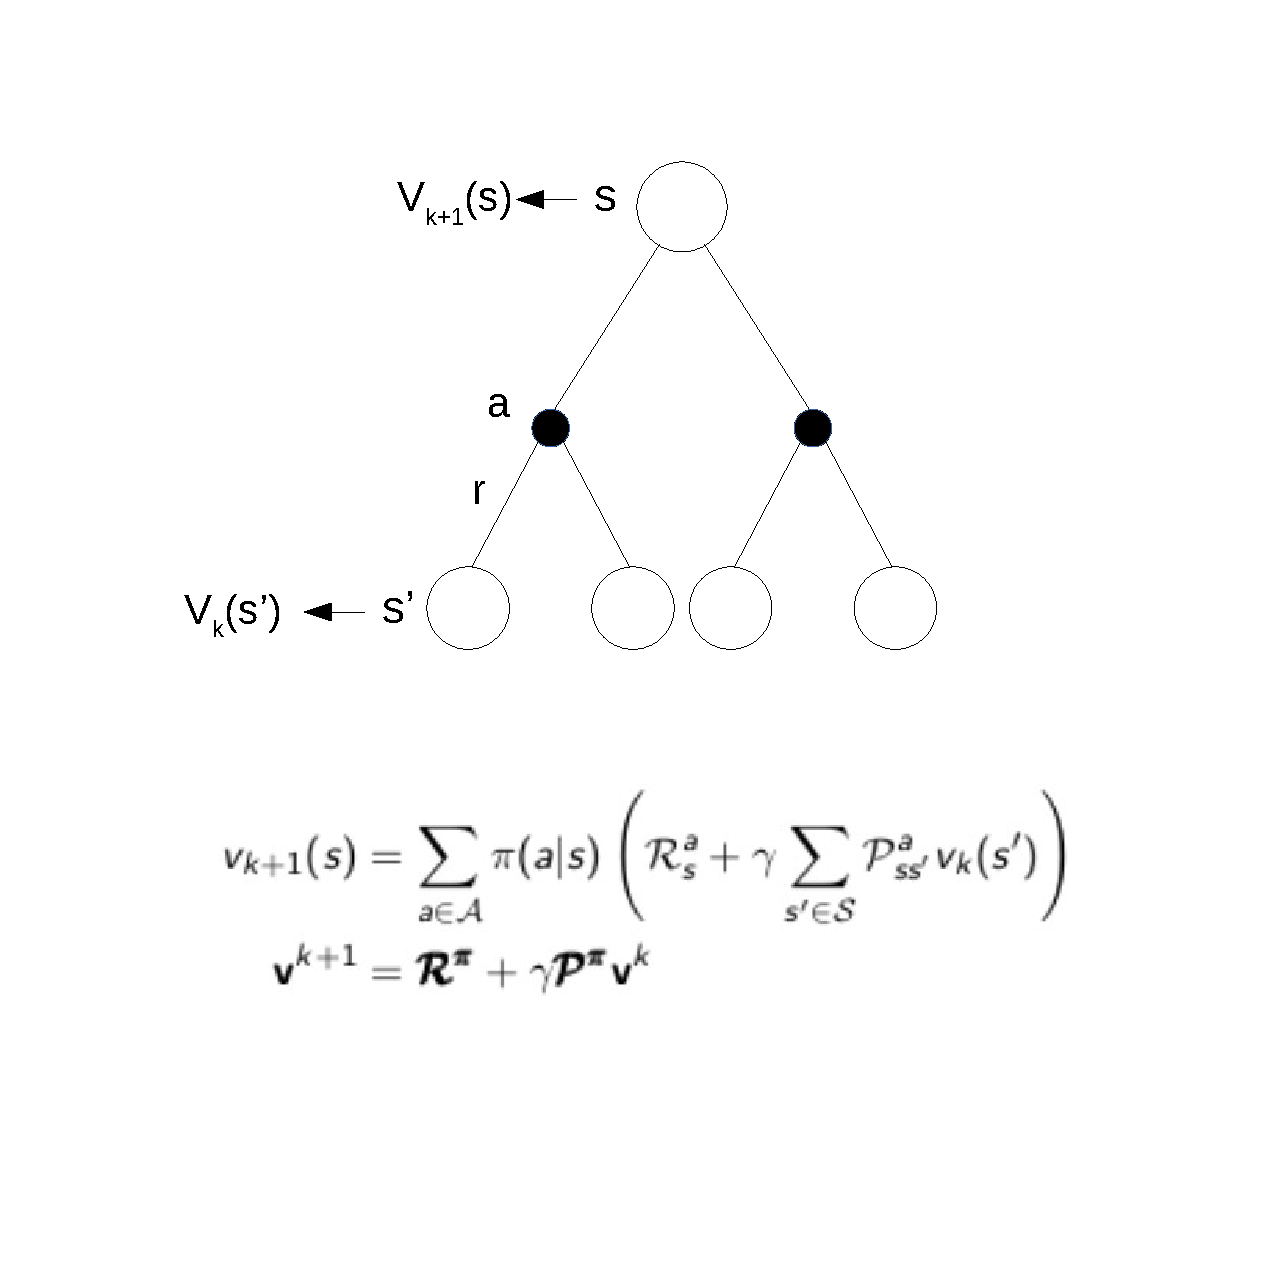
\includegraphics[width=1\linewidth]{MDP/fig/Iterative_Policy_Evaluation.pdf}
		\caption{Policy evaluation\cite{David_Silver}}
		\label{fig:iterative_policy_evaluation}
	\end{subfigure}
	\begin{subfigure}{.49\textwidth}
		\centering
		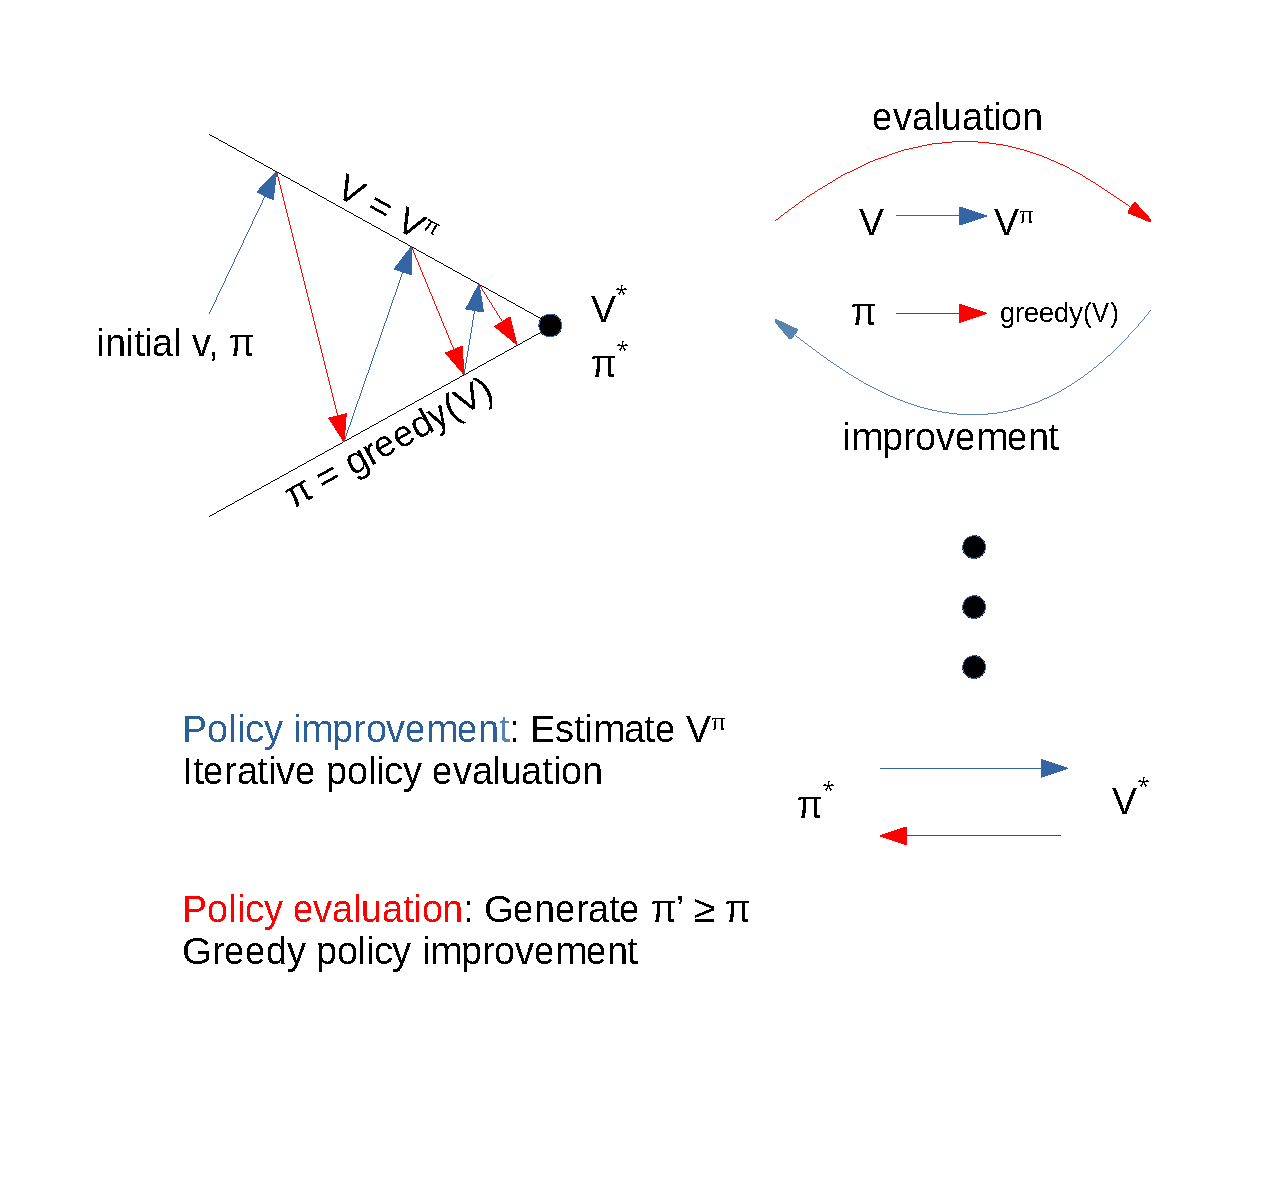
\includegraphics[width=1\linewidth]{MDP/fig/Policy_iteration.pdf}
		\caption{Greedy policy iteration visualisation\cite{David_Silver}}
		\label{fig:greedy_policy_iteration}
	\end{subfigure}
	\caption{Policy iteration with images inspired by Sutton and Barto \cite{sutton_barto}}
	\label{fig:policy_iteration}
\end{figure}

\section{Policy Improvement}

According to David Silver, a given policy $\pi$ can be improved using the following two steps \cite{David_Silver}:\\
\textbf{Step one} is \textit{evaluating} the policy $\pi$ using equation \ref{bellmanv2}: \[v_{\pi}(s) = E_{\pi}[R_{t+1} + \gamma v_{\pi}(S_{t+1})|S_t = s]\]
\textbf{Step two} is \textit{improving} the policy by acting greedy with respect to $v_\pi$ to obtain a new policy $\pi^{'}$.\\
Sutton and Barto defines acting greedy \cite{sutton_barto}, as the greedy policy which makes the agent always takes the action that looks best according to $v_\pi$ looking one step ahead, 
\begin{equation}
	\pi^{'} = greedy(v_{\pi}).
	\label{pi'}\\
\end{equation}
Sutton and Barto then further expand the greedy policy concept to consider all states and actions resulting in
\begin{equation}
	\pi^{'}(s) = \argmax\limits_{a}(R^{a}_s+\gamma\sum_{s'\in S}P^{a}_{ss'}v_*(s')) ,
	\label{pi'(s)}
\end{equation}
where $argmax_a$ denotes the action which if taken maximizes the expression following it.
By using the greedy policy, Sutton and Barto proves in \cite{sutton_barto} that we will always obtain the optimal expected return $v_*$ defined in equation \ref{bellmanv*}.\\
Sutton and Barto provides a proof that using this method always results in a policy $\pi'$ better, or as good as $\pi$, which will not be provided here but can be found in \cite{sutton_barto}. That is to say the expected return following $\pi'$ will be greater or equal than following $\pi$
\begin{equation}
	v_{\pi'} \ge v_{\pi}.
\end{equation}
In the next two sections we will use policy improvement as a tool to find the optimal policy via two methods, policy iteration and value iteration.
\section{Policy iteration}
There are two separate uses for dynamic programming in reinforcement learning. These are prediction and control which both have $(S,A,P,R,\gamma)$ as input.
\begin{itemize}
	\item The prediction method uses $(S,A,P,R,\gamma)$ and a policy $\pi$ as input, while it outputs a value function $v_\pi$. This is known as value iteration.
	\item The control method only takes $(S,A,P,R,\gamma)$ as input and outputs the optimal value function $v_*$ and optimal policy $\pi_{*}$. This is known as policy iteration.
\end{itemize}
Figure \ref{fig:greedy_policy_iteration} illustrates how greedy policy iteration works. The blue lines represents policy improvement and the red lines policy evaluation. By continuously using these two steps in succession, we eventually converge to the optimal state-value function $v_*$ and optimal policy $\pi_*$ \cite{sutton_barto}. It is known that policy iteration converges, as it uses policy improvement which we know converges from the previous section \cite{sutton_barto}.

\section{Value Iteration}
Policy iteration has a drawback of needing for every iteration, to do policy evaluation which in itself is a iterative computation requiring many calculations across the entire state-space \cite{sutton_barto}. Iterative policy evaluation only converges in the limit of its time steps. However Sutton and Barto questions if it is necessary to converge precisely on the optimal policy, or if we can stop reasonably short and acquire an approximate optimal policy \cite{sutton_barto}. They answer this by introducing the concept of value iteration, where they use policy iteration with a special case of policy evaluation as follows:
\begin{align}
	v_{k+1}(s) &= \max\limits_{a \in A}(R_s^a + \gamma\sum_{s' \in S}P_{ss'}^{a}v_k(s')) 
	\label{eq:value_iteration_summation}
\end{align}
and in vector form,
\begin{align}
	\boldsymbol{v}_{k+1} &= \max\limits_{a}(\boldsymbol{R^a} + \gamma \boldsymbol{P^a} \boldsymbol{v}_k )
	\label{eq:value_iteration_vector}
\end{align}
Note these equations are the Bellman optimality equation (in equation \ref{bellmanv*}), turned into an update rule.
In the next chapter we use almost the same method to find the optimal policy, except that we do not assume that we have access to a perfect model of the MDP.
\section{Value iteration grid-world example problem}
\begin{figure}[!htb]
	\centering
	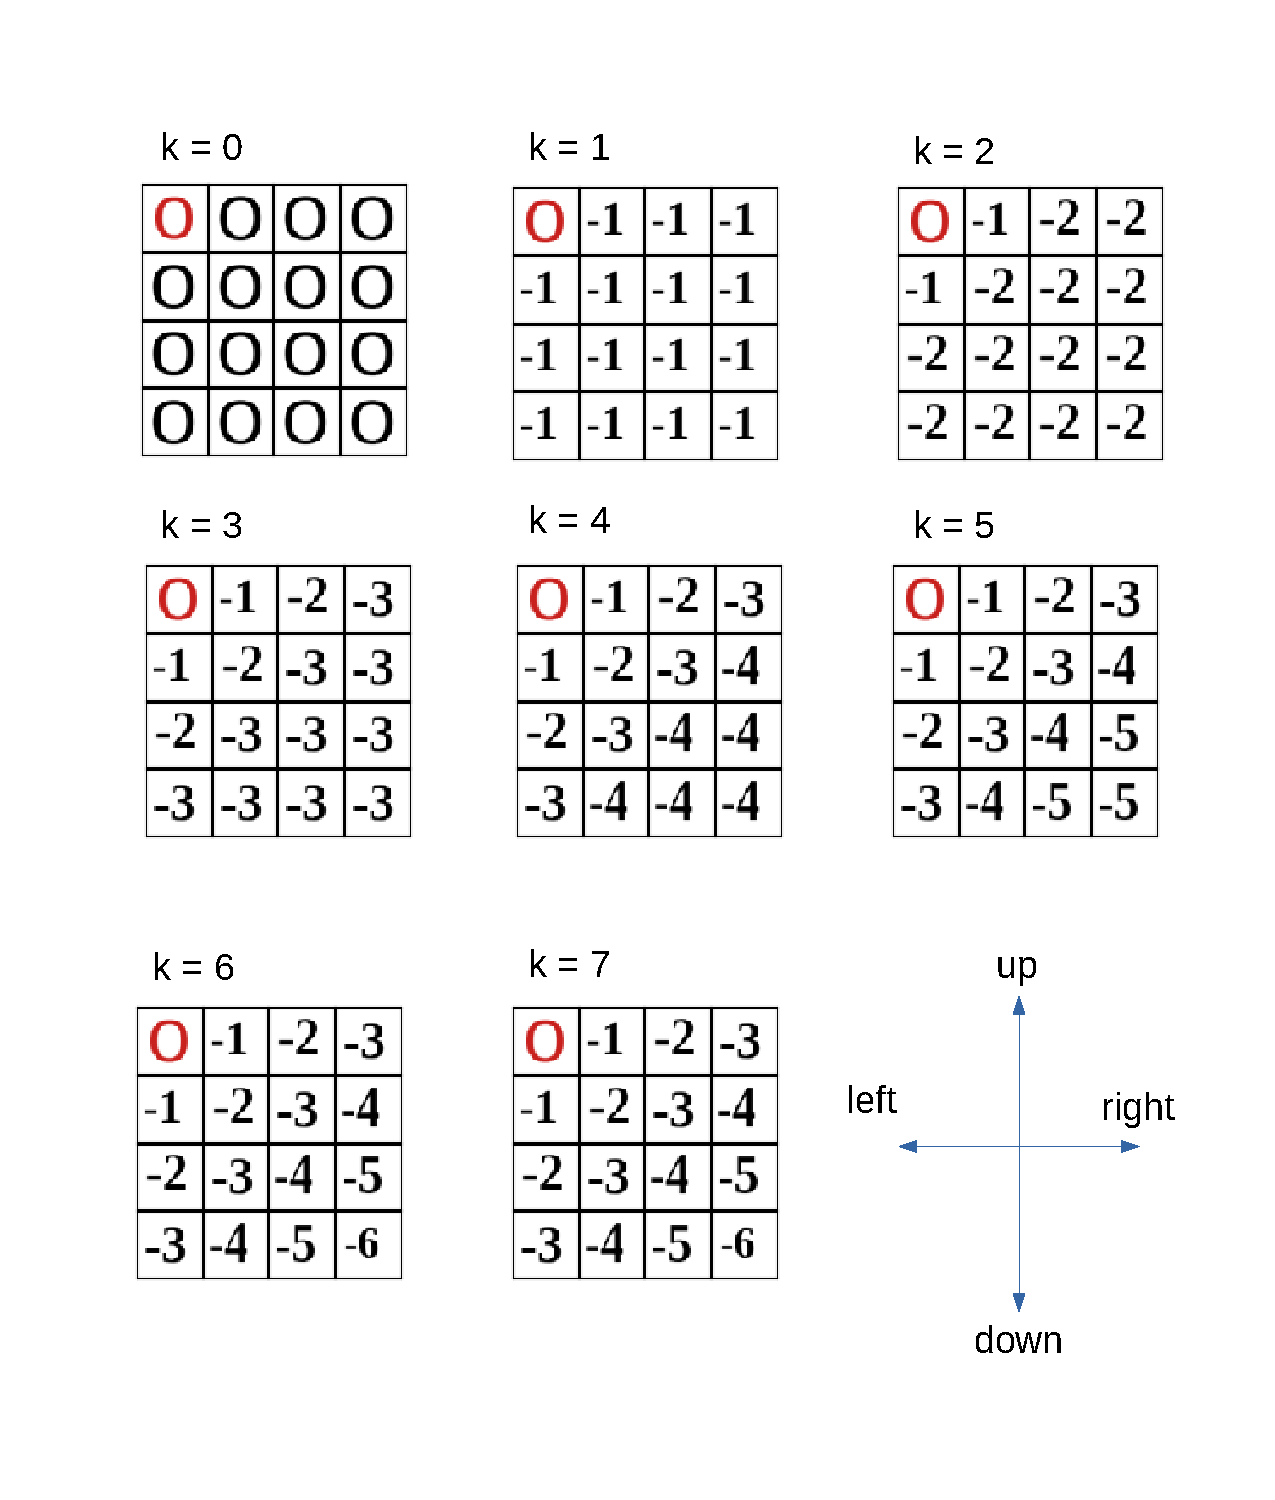
\includegraphics[width=0.5\linewidth]{Dynamic_Programming/fig/value_iteration_grid_world.pdf}
	\caption{This is a grid world example solved using value iteration. The goal is to have values in the cells represent the amount of steps it would take from that cell to the cell in the top left corner of that iteration. Each step results in a reward of -1. All iterations after iteration k = 7 are the same, although not shown, as the optimal state-value function $v_7(s) = v_*(s)$ has been reached by then.}
	\label{fig:grid_world}
\end{figure}
\noindent Figure \ref{fig:grid_world} is an example problem, which David Silver \cite{David_Silver} uses to illustrate how value iteration works. The states are defined as cells contained within a grid. The example in Figure \ref{fig:grid_world} has a state space of 16 states with S $\in$ [0,15] and an action space of actions A = \{up, down, left, right, NONE\} indicated on the figure. The action NONE is used to indicate the agent choosing to stay in its current state. Each state consists of an index and a value, with the terminal state being at index 0. The agent can move in all directions in all states, except for the terminal state, where it can only choose to stay still. The state indices are numbered from left to right and top to bottom in ascending order starting at 0. Hence we can treat the states as an array in computer programming with 0 to 3 being the top row indices, 3 to 7 the second most top row indices etc.

Imagine that we have an agent dropped into a grid as is shown in the initial iteration in Figure \ref{fig:grid_world} then
\begin{equation}
	v_0(0) = v_0(1) = v_0(2) = v_0(3) = v_0(4) = ... = v_0(s) = 0.
\end{equation}
Hence at iteration 0 no matter which state the agent is dropped into, all actions are equally valuable to it. As the iterations k increases, $v_k(s) \rightarrow v_*(s)$. We know the agent has learnt the optimal state-value function, when the current iterations state-value function has a negligible, or no difference from its previous iteration 
\begin{equation}
	v_{k+1}(s) - v_k(s) \le \delta ,
\end{equation}
where $\delta$ is a chosen threshold.